\section{Άσκηση 4}
\subsection{Θεωρητική Ανάλυση}
Σε αυτήν την άσκηση θα θεωρήσουμε ότι μπορούμε να μετρήσουμε μόνο τη θέση του κινητήρα. Γιάυτό, θα σχεδιάσουμε ένα
σύστημα εκτίμησης των μεταβλητών κατάστασης του συστήματος. Θα πρέπει, λοιπόν, να ελέγξουμε αν το σύστημά μας είναι παρατηρήσιμο. Υπενθυμίζουμε ότι οι πίνακες του συστήματός μας είναι οι
\begin{align*}
	A &= \begin{bmatrix} -\frac{1}{T_m} & 0 \\ k_μk_0 & 0\end{bmatrix} \\
	B &= \begin{bmatrix} \frac{k_m}{T_m} \\ 0 \end{bmatrix} \\
	C &= \begin{bmatrix} 0 & 1\end{bmatrix} \\
	D &= \begin{bmatrix} 0 \end{bmatrix}
\end{align*}
Και το χαρακτηρηστικό πολυώνυμο $det(sI - A) = s^2 + \dfrac{1}{T_m}s = s^2 + a_1s+a_2$

Οπότε ο πίνακας παρατηρησιμότητας είναι ο
\[
    W = 
    \begin{bmatrix}
        C \\ CA
    \end{bmatrix} = 
    \begin{bmatrix}
        0 & 1 \\
        k_μk_0 & 0
    \end{bmatrix}
\]
Επειδή $det(W) = -k_μk_0 = -5.22 \cdot 10^{-3} \neq 0$, το σύστημα είναι παρατηρήσιμο. Έχουμε γραμμικό παρατηρήσιμο σύστημα, άρα αν $\hat{x}$ η εκτίμηση και $\tilde{x} = x - \hat{x}$ το σφάλμα της εκτίμησης, ο παρατηρητής μας θα είναι της μορφής
\[
    \dot{\hat{x}} = A\hat{x} + Bu + L(y-C\hat{x})
\]
Με διαφορική εξίσωση σφάλματος
\[
    \dot{\tilde{x}} = (A - LC)\tilde{x}
\]
Όπου
\[
    L = W^{-1}\tilde{W}
    \begin{bmatrix}
        p_1 - a_1 \\ p_2 - a_2
    \end{bmatrix} = 
    W^{-1}\tilde{W}
    \begin{bmatrix}
        p_1 - \frac{1}{T_m} \\ p_2 - 0
    \end{bmatrix}
\]
Και
\[
    \tilde{W} = \begin{bmatrix}
        1 & 0 \\ a_1 & 1
    \end{bmatrix}^{-1} = 
    \begin{bmatrix}
        1 & 0 \\ \frac{1}{T_m} & 1
    \end{bmatrix}^{-1}
\]
Έπειτα από πράξεις, έχουμε τελικά
\[
    L = \begin{bmatrix}
        -407.47p_1+866.96+191.57p_2 \\ p_1 - 2.13
    \end{bmatrix} = 
    \begin{bmatrix}
        L_1 \\ L_2
    \end{bmatrix}
\]
Σημαντικό είναι να σημειώσουμε ότι τα $p_1, p_2$ υπολογίζονται από το επιθυμητό χαρακτηριστικό πολυώνυμο του παρατηρητή. Συγκεκριμένα, από το $s^2 + p_1s + p_2$. Αλλάζοντας τους πόλους $s_1, s_2$ αυτού του πολυωνύμου, αλλάζουν και τα $p_1, p_2$, αφού $p_1 = -s_1 - s_2$ και $p_2 = s_1s_2$. Φυσικά, για να έχουμε ευστάθεια πρέπει από κριτήριο Routh-Hurwitz να ισχύει $p_1 > 0$ και $p_2 > 0$.

Στο Ερώτημα 2 μας ζητείται να σχεδιαστεί ελεγκτής γραμμικής ανάδρασης εξόδου, οπότε θα χρησιμοποιήσουμε τον $u=-k\hat{x} + k_rr$ με κέρδη όπως αναγράφονται παρακάτω.
\subsection{Εργαστηριακά Αποτελέσματα}
\subsubsection{Ερώτημα 1}
Για $s_1 = -3,\ s_2 = -10$ (δηλαδή $L_1 = 1316.95,\ L_2 = 27.87$) έχουμε τα παρακάτω αποτελέσματα. Οι εκτιμήσεις είναι με πορτοκαλί, ενώ οι πραγματικές μετρήσεις με μπλε. Παρατηρούμε ότι η εκτίμηση της θέσης είναι αρκετά ικανοποιητική (αναμενόμενο αφού αυτήν θεωρήσαμε ότι μπορούμε να μετρήσουμε), ενώ η εκτίμηση της ταχύτητας «δυσκολέυεται» λίγο να βρει και να διατηρήσει την πραγματική τιμή. Πάντως, οι μεγάλες πτώσεις της εκτιμώμενης ταχύτητας ανά 1 περίπου δευτερόλεπτο οφείλονται στο σφάλμα θέσης που προκαλείται από το «κενό» του ποτενσιόμετρου. Για τον μηδενισμό της πραγματικής τιμής της θέσης από την άλλη, ευθύνεται ο ελαττωματικός κινητήρας που μελετάμε.
\begin{figure}[H]
    \centering
    \begin{minipage}{0.45\textwidth}
        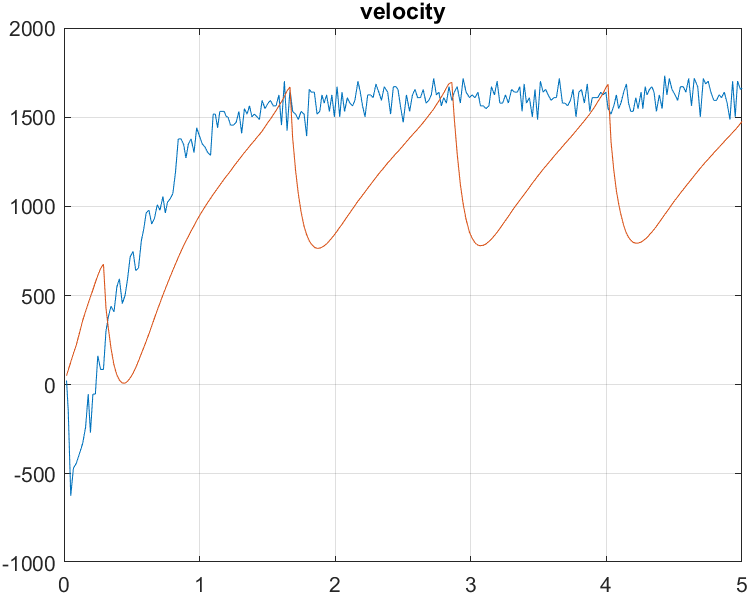
\includegraphics[width=\linewidth]{Images/lab4/1/kalo/vel421.png}
    \end{minipage}
    \hfill
    \begin{minipage}{0.45\textwidth}
        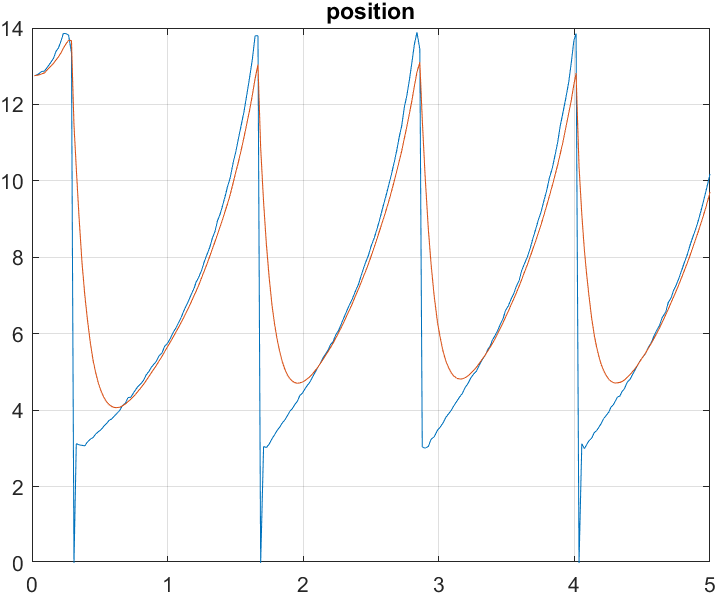
\includegraphics[width=\linewidth]{Images/lab4/1/kalo/pos421.png}
    \end{minipage}
\end{figure}
\begin{figure}[H]
    \centering
    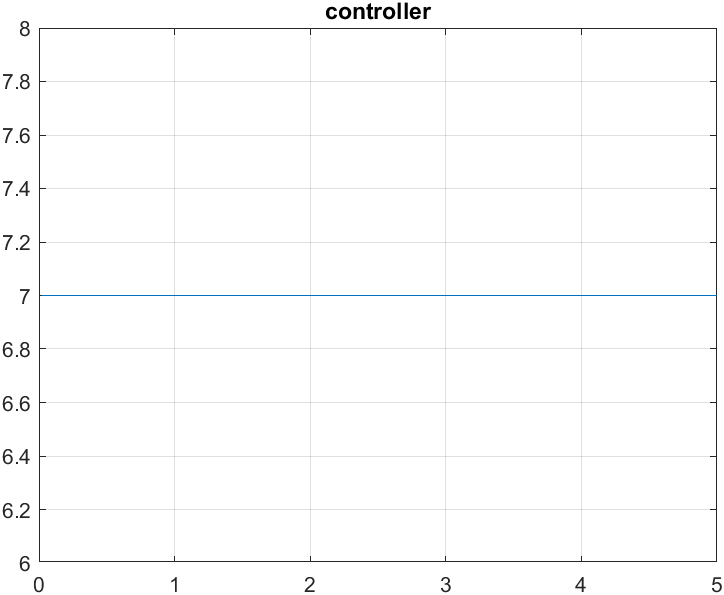
\includegraphics[width=0.5\linewidth]{Images/lab4/1/kalo/con421.png}
\end{figure}
Ενδιαφέρον παρουσιάζουν τα αποτελέσματα αν μετακινήσουμε τον έναν πόλο λίγο πιο αριστερά στο μιγαδικό επίπεδο. Συγκεκριμένα, για $s_1 = -3,\ s_2 = -25$ (δηλαδή $L_1 = 3825,55,\ L_2 = 72,87$) βλέπουμε παρακάτω αλλαγές τόσο στην ταχύτητα όσο και στην θέση. Όσον αφορά τη θέση, η εκτίμηση μας έχει σημαντική βελτίωση απο πριν. Πλέον είναι πολύ πιο πιστή στην πραγματική τιμή. Η ταχύτητα, από την άλλη, δεν διατηρεί τόσο καλά την πραγματική τιμή όσο πριν. Ωστόσο, την ακολουθεί πιο γρήγορα και με μικρότερο σφάλμα στην αρχή. Εν ολίγοις, ο πρώτος παρατηρητής ταχύτητας έχει πιο «μαλακή» απόκριση, αλλά θυσιάζει την ταχύτητα σύγκλισης, ενώ ο δεύτερος έχει γρήγορη εκτίμηση, αλλά όχι τόσο καλή διατήρηση στην συνέχεια.

\begin{figure}[H]
    \centering
    \begin{minipage}{0.45\textwidth}
        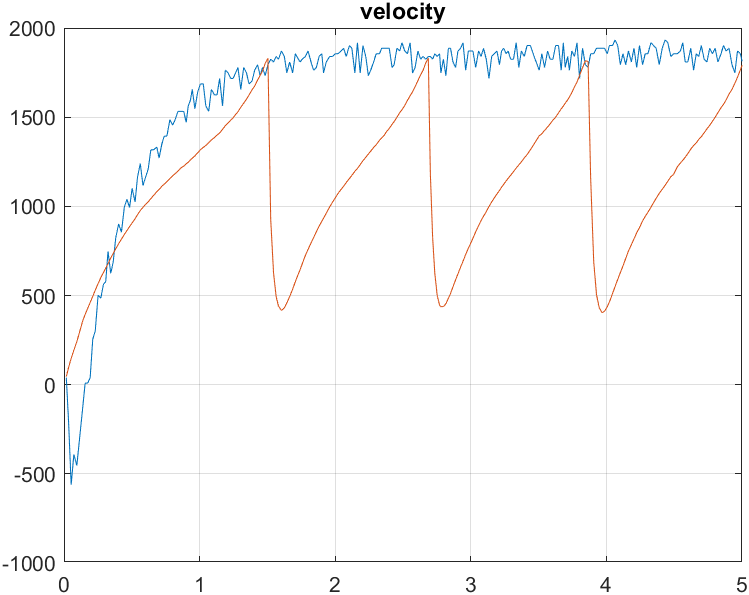
\includegraphics[width=\linewidth]{Images/lab4/1/ligo xeirotero/vel.png}
    \end{minipage}
    \hfill
    \begin{minipage}{0.45\textwidth}
        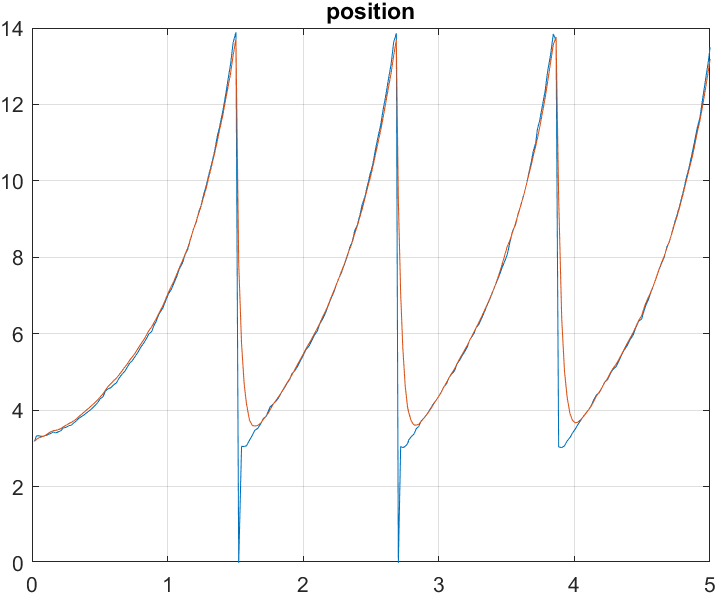
\includegraphics[width=\linewidth]{Images/lab4/1/ligo xeirotero/pos.png}
    \end{minipage}
\end{figure}
Πάντως, η βέλτιστη απόκριση δόθηκε για $s_1 = -20,\ s_2 = -50$  (δηλαδή $L_1 = 163914.06,\ 55, L_2 = 67.87$). Με αυτους τους πολύ αρνητικούς πόλους, η ταχύτητα διατηρεί για πολύ μεγαλύτερο χρονικό διάστημα την πραγματική τιμή, αν και παρατηρούμε ότι σε κάποιες χρονικές τιμές την ξεπερνάει κιόλας. Η εκτίμηση της θέσης είναι λίγο χειρότερη, αλλά αποδεκτή. Γενικώς για $u=7$ είναι η καλύτερη απόκριση που πετύχαμε, αλλά το μειονέκτημά της φαίνεται στο επόμενο ερώτημα.
\begin{figure}[H]
    \centering
    \begin{minipage}{0.45\textwidth}
        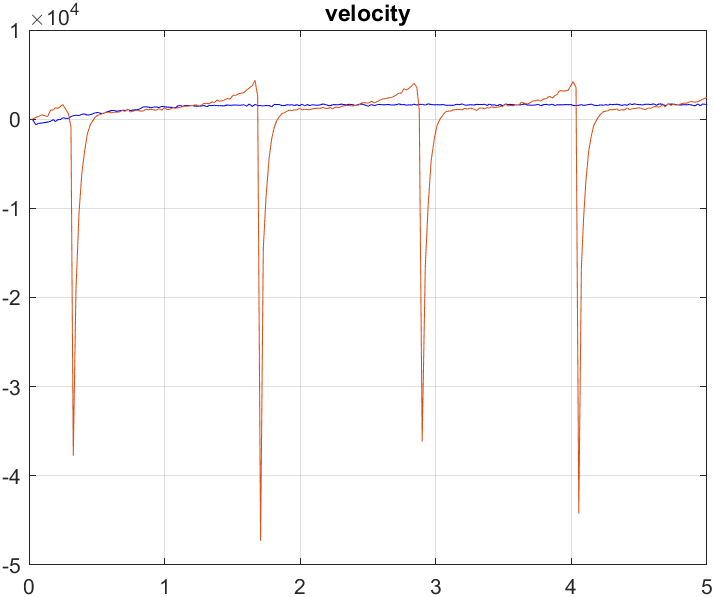
\includegraphics[width=\linewidth]{Images/lab4/1/veltisto/vel4.1.png}
    \end{minipage}
    \hfill
    \begin{minipage}{0.45\textwidth}
        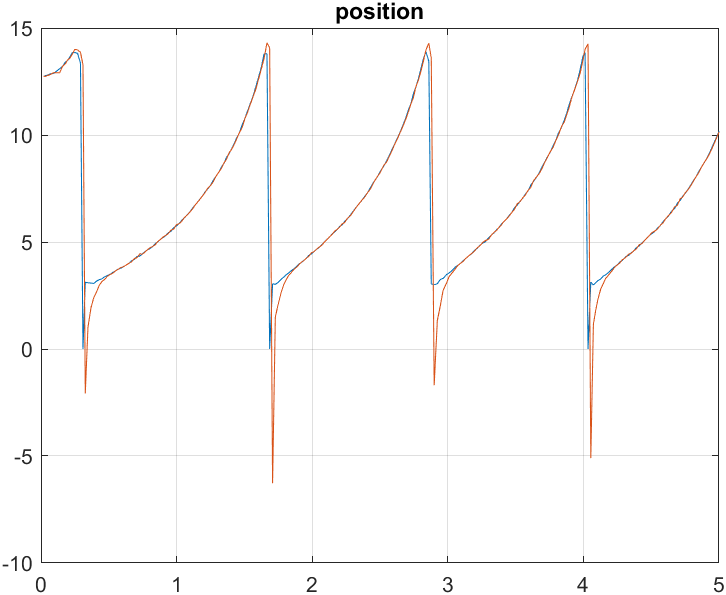
\includegraphics[width=\linewidth]{Images/lab4/1/veltisto/pos4.1.png}
    \end{minipage}
\end{figure}
\subsubsection{Ερώτημα 2}
Έπειτα από πληθώρα δοκιμών για τα ιδανικά κέρδη, καταλήξαμε στα $k_1 = 0.005,\ k_2 = k_r = 5$, ενώ οι πόλοι διατηρήθηκαν στο $s_1 = -3,\ s_2 = -10$. Η εκτίμησή μας είναι αρκετά καλή, αν και δεν απουσιάζει το σφάλμα σε αυτήν, πιο εμφανές στην ταχύτητα. Υπενθυμίζουμε ότι λόγω ελαττωματικού κινητήρα έχουμε $θ_0 = 5V$ και $θ_{ref} = 8V$. Αναφορικά με την ερώτηση περί αλλαγής των πόλων του παρατηρητή $s_1,\ s_2$ και διατήρησης των πόλων (δηλαδή των κερδών) του ελεγκτή $u$ μας, μπορόυμε να σχολιάσουμε ότι όσο μετακινούμε προς τα αριστερά του μιγαδικού επιπέδου τους πόλους του παρατηρητή μας έχουμε ταχύτερη απόκριση. Αυτό, όμως, κάνει τον ελεγκτή πιο ευαίσθητο στον θόρυβο, αφού οποιοδήποτε σφάλμα, όπως θόρυβος μέτρησης, ενισχύεται περισσότερο στην εκτίμηση. Από την άλλη, οι λιγότερο αρνητικοί πόλοι είναι μεν πιο ανθεκτικοί και σταθεροί στις εκτιμήσεις τους, αλλά παρέχουν πιο αργή σύγκλιση. Τελικά, ανάλογα με τις εκάστοτε απαιτήσεις του σχεδιαστή επιλέγονται και οι κατάλληλοι πόλοι.

\begin{figure}[H]
    \centering
    \begin{minipage}{0.45\textwidth}
        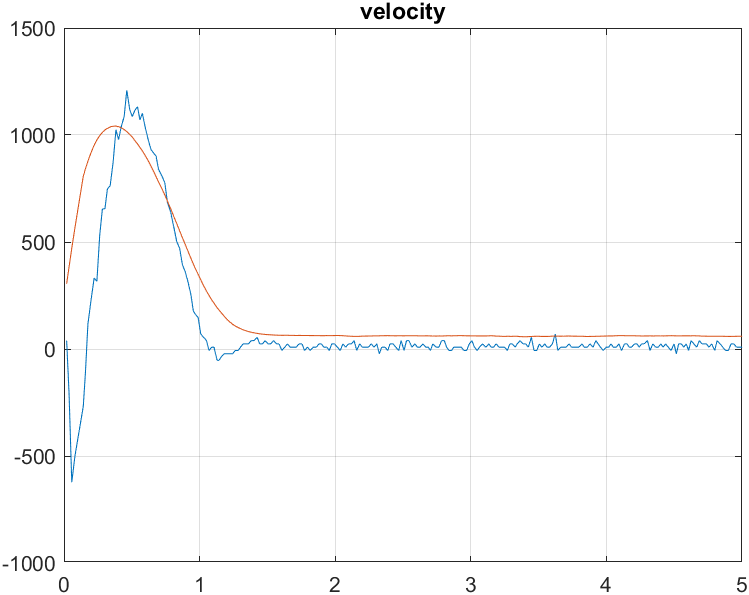
\includegraphics[width=\linewidth]{Images/lab4/2/vel422.png}
    \end{minipage}
    \hfill
    \begin{minipage}{0.45\textwidth}
        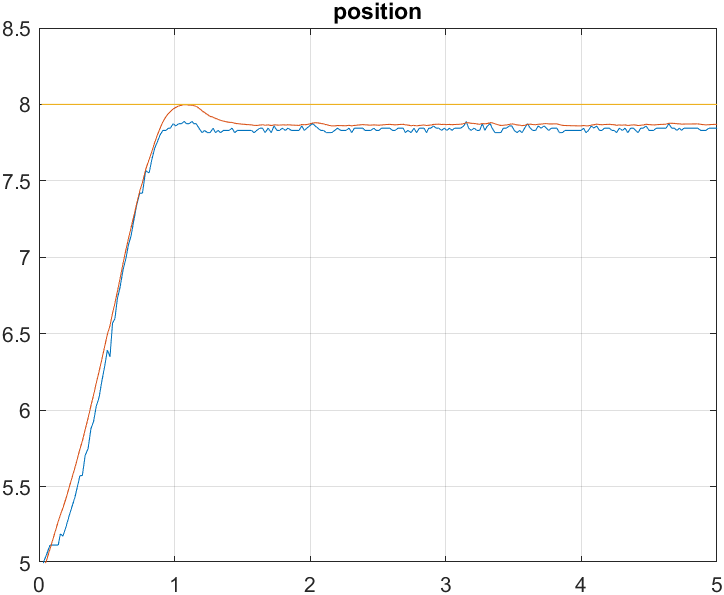
\includegraphics[width=\linewidth]{Images/lab4/2/pos422.png}
    \end{minipage}
\end{figure}
\begin{figure}[H]
    \centering
    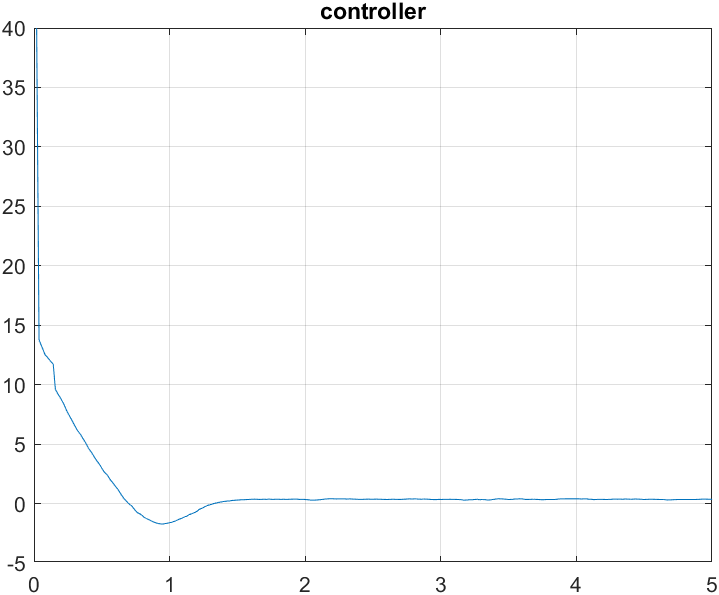
\includegraphics[width=0.5\linewidth]{Images/lab4/2/con422.png}
\end{figure}
Τα παραπάνω επιβεβαιώνονται απο τα ακόλουθα αποτελέσματα για $s_1 = -20,\ s_2 = -50$ και $k_1 = 0.005,\ k_2 = k_r = 5$, όπου αν και οι εκτιμήσεις είναι πολύ καλές, καλύτερες από πριν, βλέπουμε ότι ιδιαίτερα στην ταχύτητα υπάρχουν πολλά «σκαμπανεβάσματα» που προέρχονται από την ενίσχυση του θορύβου λόγω των πολύ αρνητικών πόλων του παρατηρητή.
\begin{figure}[H]
    \centering
    \begin{minipage}{0.45\textwidth}
        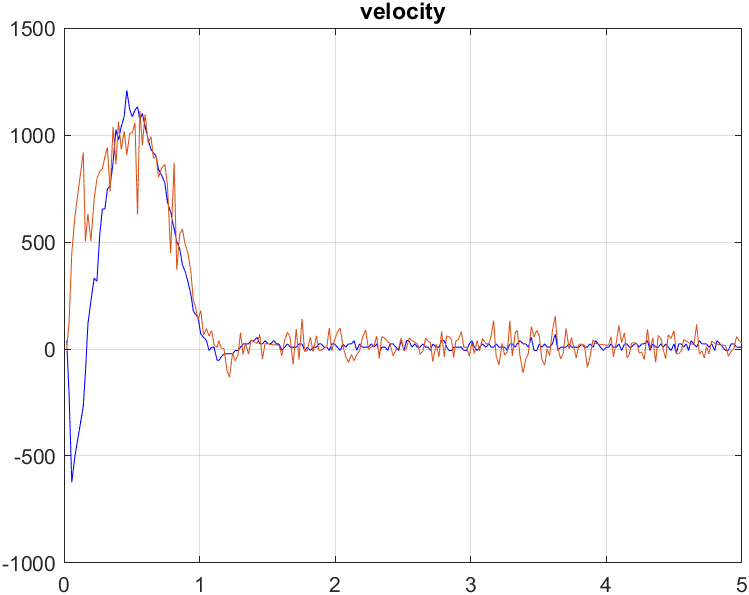
\includegraphics[width=\linewidth]{Images/lab4/2/vel4.2.png}
    \end{minipage}
    \hfill
    \begin{minipage}{0.45\textwidth}
        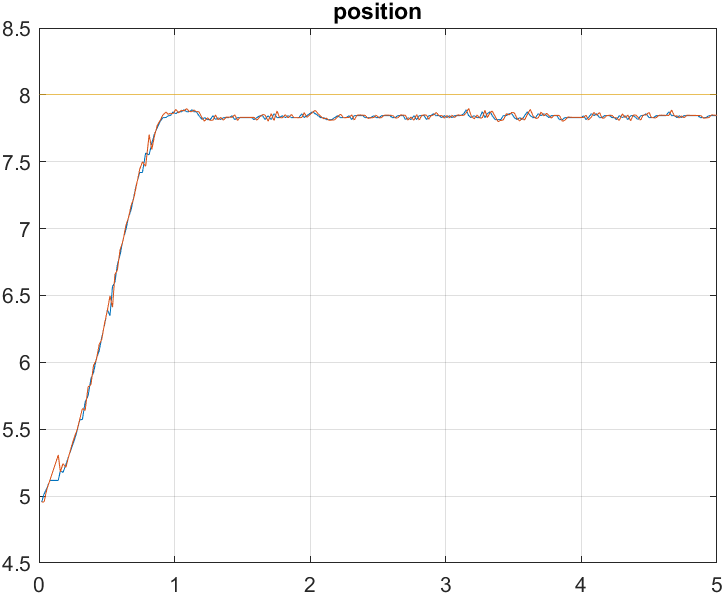
\includegraphics[width=\linewidth]{Images/lab4/2/pos4.2.png}
    \end{minipage}
\end{figure}
\begin{figure}[H]
    \centering
    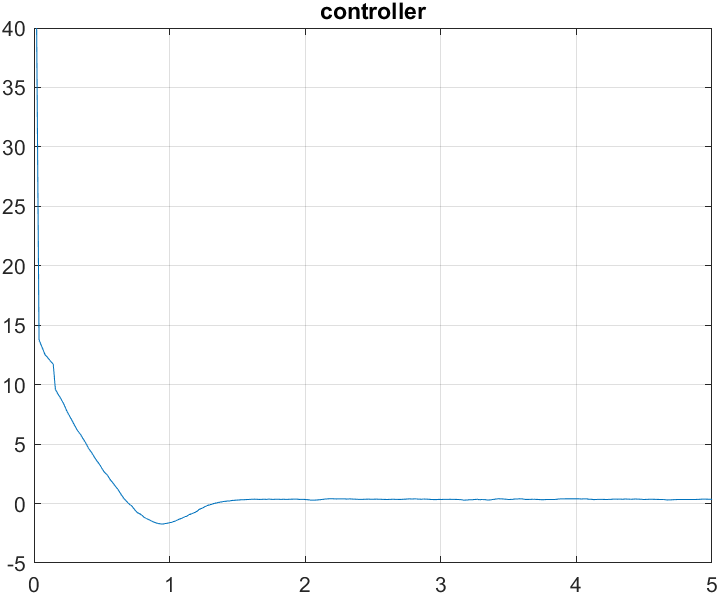
\includegraphics[width=0.5\linewidth]{Images/lab4/2/con4.2.png}
\end{figure}